\chapter{Introduction}

The openSUSE KIWI Image System provides a complete operating system
image solution for Linux supported hardware platforms as well as
for virtualisation systems like Xen, VMWare, etc. The KIWI architecture
was designed as a two level system. The first stage, based on a valid
\textbf{software package source}, creates a so called \textbf{unpacked image}
according to the provided image description. The second stage creates from
a required unpacked image an operating system image. The result of the
second stage is called a \textbf{packed image} or short an image.

\begin{figure}[h]
\centering
\includegraphics[scale=0.5]{pictures/intro.eps}
\caption{Image Serving Architecture}
\label{fig:architecture}
\end{figure}

Because this document contains conceptual information about an image system,
it is important to understand what an operating system image is all about.
A normal installation process is starting from a given installation source
and installs single pieces of software until the system is complete. During
this process there may be manual user intervention required. However an
operating system image represents an already completed \textit{installation}
encapsulated as a file and optionally includes the configuration for a
specific task. Such an operating system starts working as soon as the
image has been brought to a system storage device no matter if this is a
volatile or non volatile storage. The process of creating an image takes
place without user interaction.
This means all requirements of the encapsulated system has to be fulfilled
before the image is created. All of this information is stored in the
\textbf{image description}.
